\section{Xử lý dữ liệu}
\subsection{Mô tả dữ liệu}
\begin{itemize}
    \item Bộ dữ liệu: Fashion Product Images (Small)
    \item Độ lớn: 593MB
    \item Mô tả: Chứa các hình ảnh thuộc về lĩnh vực thời trang như quần áo, phụ kiện, giày dép
    \item Được lấy trên Kaggle : \href{https://www.kaggle.com/datasets/paramaggarwal/fashion-product-images-small}{https://www.kaggle.com/datasets/paramaggarwal/fashion-product-images-small}
    \item Bộ dữ liệu gồm có:
    \begin{itemize}
        \item Hơn 44000 hình ảnh sản phẩm:
        \begin{itemize}
            \item Có cùng kích thước là 60x80
            \item Tên của mỗi hình ảnh đó chính là cái để xác định thông tin của nó trong file nhãn dữ liệu.
        \end{itemize}
        \begin{center}
            \begin{figure}[!h]
                \centering
                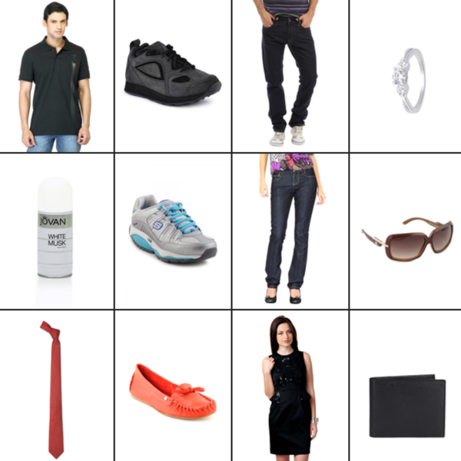
\includegraphics[scale = 0.9]{fileanh/43.png}
                \caption{Hình ảnh sản phẩm}
            \end{figure}
        \end{center}
        \newpage

        \item File nhãn dữ liệu : \textbf{styles.csv}
        \begin{center}
            \begin{figure}[!h]
                \centering
                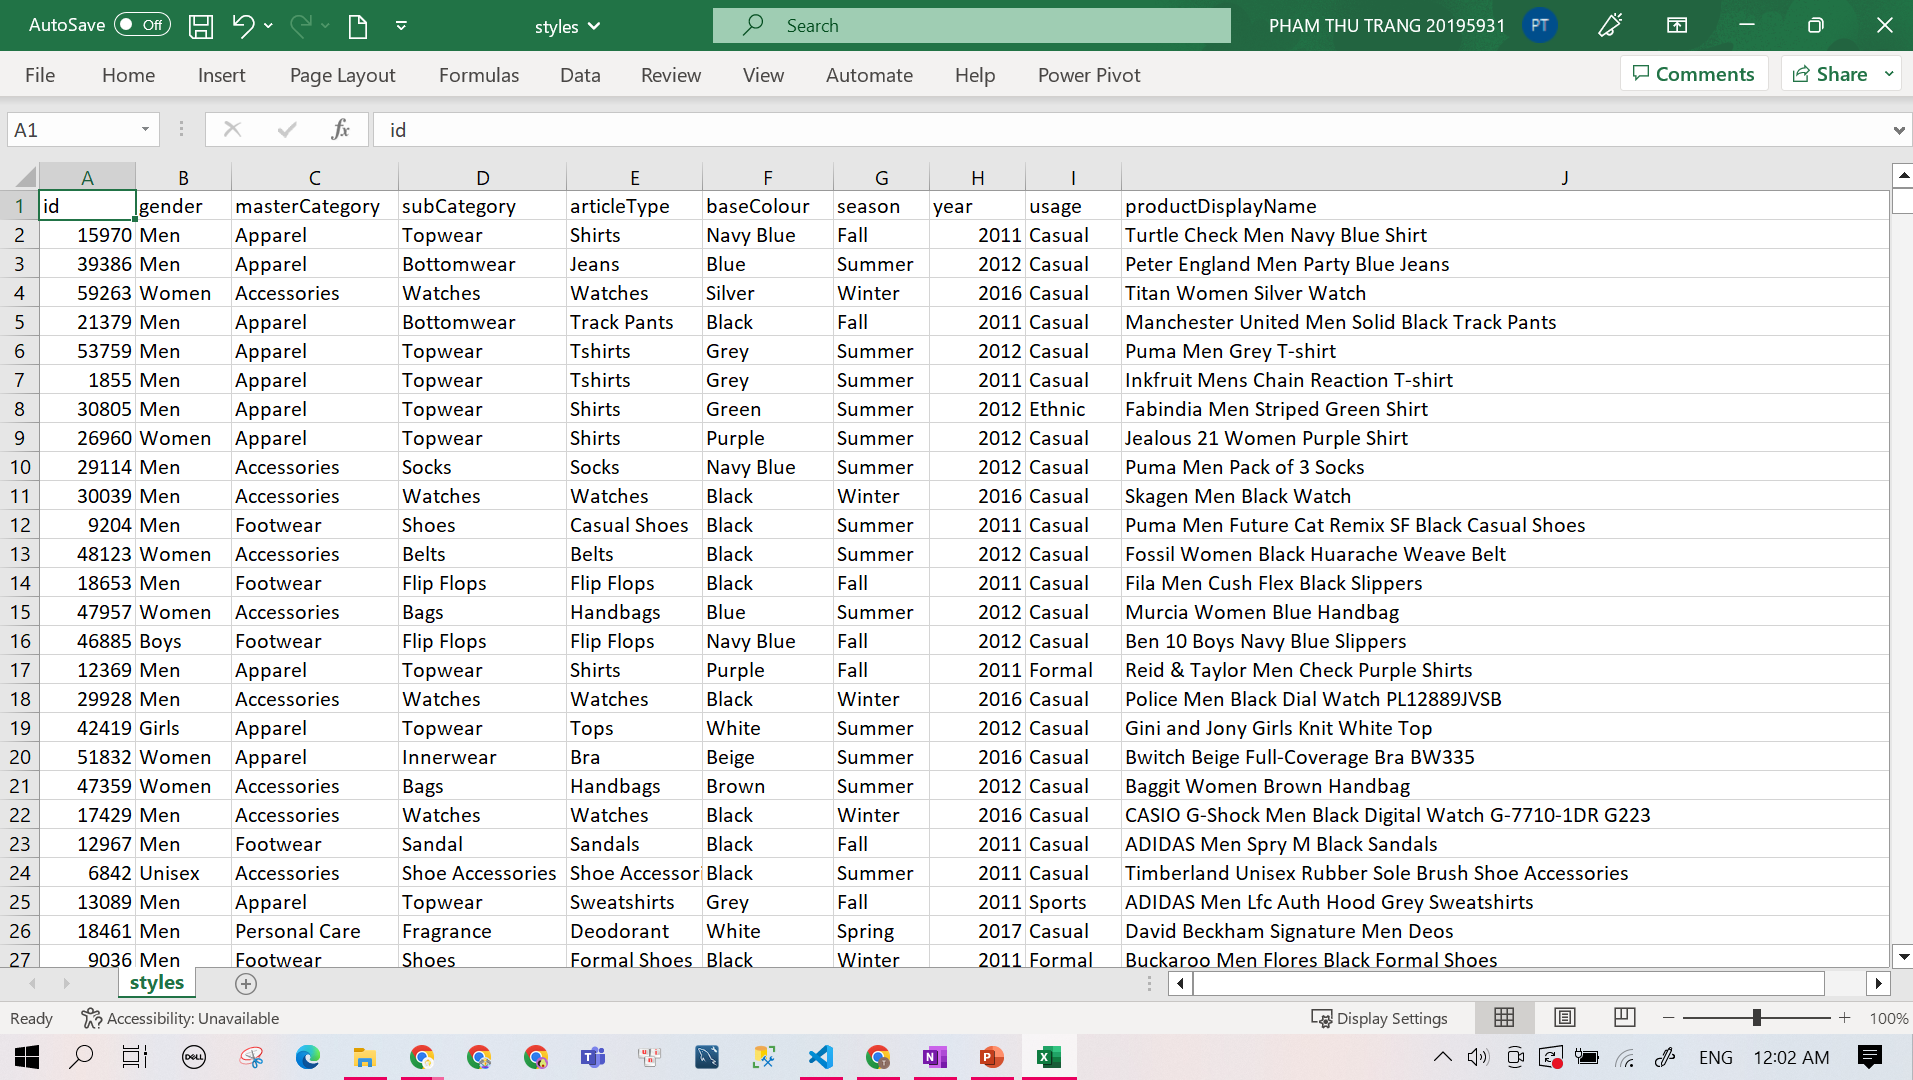
\includegraphics[scale = 0.25]{fileanh/1.png}
                \caption{Bảng mô tả thông tin các hình ảnh}
            \end{figure}
        \end{center}

        \item Hình ảnh trực quan
        \begin{center}
            \begin{figure}[!h]
                \centering
                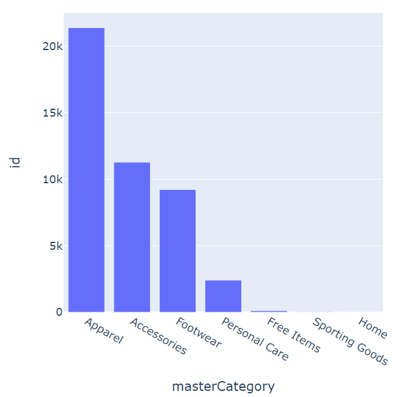
\includegraphics[scale = 0.9]{fileanh/2.png}
                \caption{Số lượng mỗi thuộc tính của cột masterCategory}
            \end{figure}
        \end{center}
        \newpage
        \begin{center}
            \begin{figure}[!h]
                \centering
                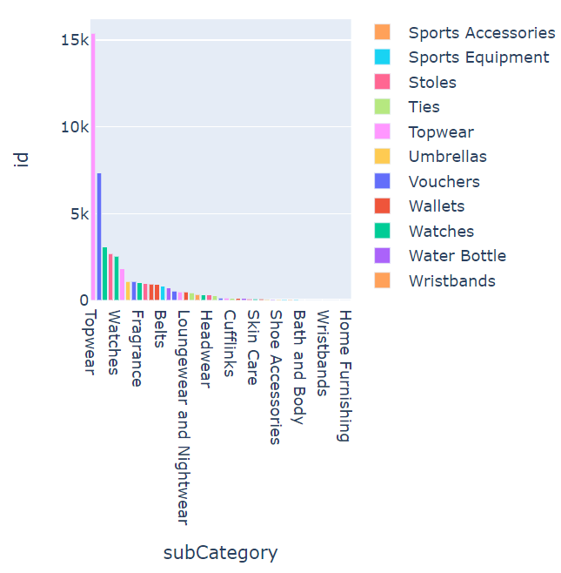
\includegraphics[scale = 1]{fileanh/3.png}
                \caption{Số lượng mỗi thuộc tính của cột subCategory}
            \end{figure}
        \end{center}
        
    \end{itemize}
\end{itemize}

\newpage
\subsection{Tiền xử lý dữ liệu}
Thuộc tính \textbf{masterCategory} gồm có 7 lớp, cụ thể:
\begin{center}
            \begin{figure}[!h]
                \centering
                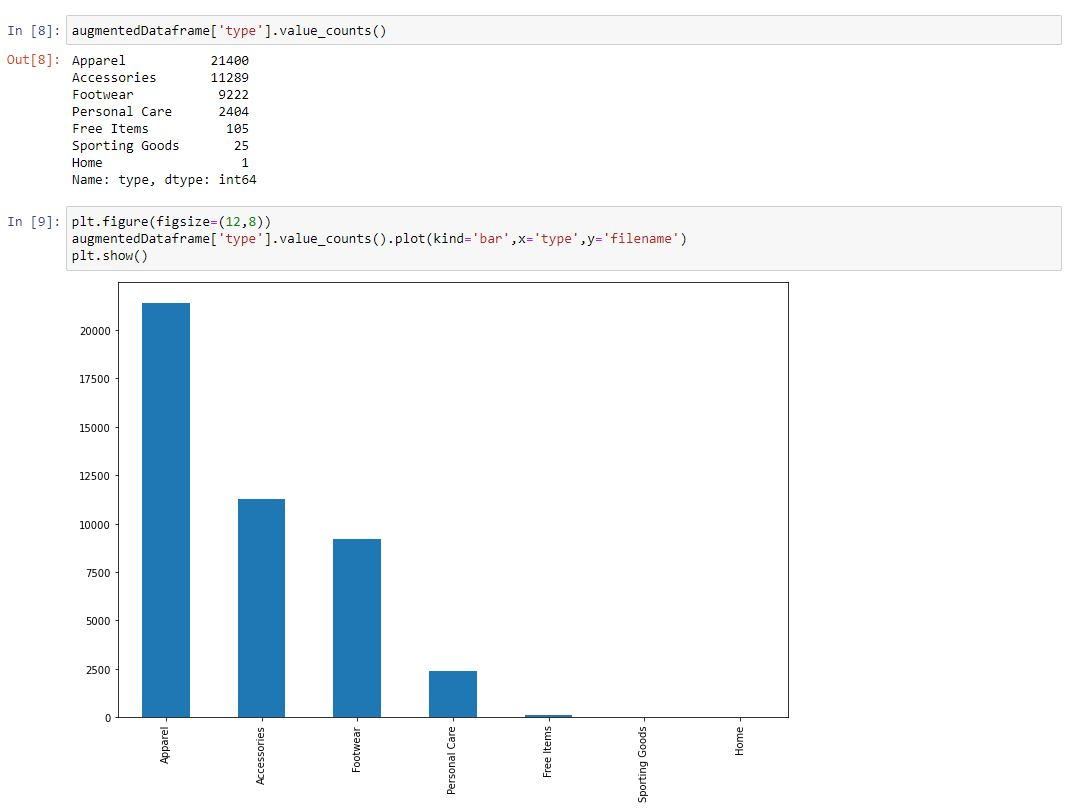
\includegraphics[scale = 0.85]{fileanh/4.jpg}
                \caption{Thông tin của cột masterCategory}
            \end{figure}
        \end{center}
\begin{remark}
    Một số lớp có số lượng quá ít nên sẽ bị loại bỏ và sẽ chỉ giữ lại 3 lớp có số lượng cao nhất trở thành 3 lớp chính cho bài toán.
\end{remark}

\subsubsection{Loại bỏ các lớp không sử dụng}
\begin{lstlisting}[language = python]
data = df.copy()
for i in range(0,total_row,1):
  if df['masterCategory'][i] == 'Personal Care':
    data = data.drop(labels = i, axis =0 )
    os.remove(DATASET_PATH+list_directory[index]+"/"+df.loc[i,'image'])
  elif df['masterCategory'][i] == 'Free Items':
    data = data.drop(labels = i, axis =0 )
    os.remove(DATASET_PATH+list_directory[index]+"/"+df.loc[i,'image'])
  elif df['masterCategory'][i] == 'Sporting Goods':
    data = data.drop(labels = i, axis =0 )
    os.remove(DATASET_PATH+list_directory[index]+"/"+df.loc[i,'image'])
  elif df['masterCategory'][i] =='Home':
    data = data.drop(labels = i, axis =0 )
    os.remove(DATASET_PATH+list_directory[index]+"/"+df.loc[i,'image'])
\end{lstlisting}

\subsubsection{Kiểm tra số lượng hình ảnh và kích thước của dataframe}
\begin{lstlisting}[language = python]
data_path = "C:/Users/admin/3D Objects/Khaiphadulieu/archive/myntradataset/images"
print(len(os.listdir(data_path)))
\end{lstlisting}
41906

\begin{lstlisting}[language = python]
data.shape
\end{lstlisting}
(41911, 11)

\begin{remark}
Số lượng hình ảnh hiện có và số lượng dòng thông tin của các ảnh trong file nhãn là khác nhau.
\end{remark}


\subsubsection{Thống nhất số lượng hình ảnh với file nhãn}
Danh sách các hình ảnh bị thừa/thiếu
\begin{lstlisting}[language = python]
#Su dung khi file anh > so row trong styles.csv
#for i in range(0,total,1):
#  if os.listdir(data_path)[i] not in listt :
#    path = DATASET_PATH+list_directory[index]+"/"+os.listdir(data_path)[i]    
#    shutil.move(path,'C:/Users/admin/3D Objects/Khaiphadulieu/archive/')


#Su dung khi file anh < so row trong styles.csv
path_del = []
for i in range(0,total,1):
    if listt[i] not in os.listdir(data_path):
        #print(listt[i])
        path_del.append(listt[i])
print(path_del)
\end{lstlisting}
['39403.jpg', '39410.jpg', '39401.jpg', '39425.jpg', '12347.jpg']\\

Xóa các dòng trong file nhãn bị thừa
\begin{lstlisting}[language = python]
for i in path_del:
    data = data.drop(data[data['image'] == i].index)
data.shape
\end{lstlisting}
(41906, 11)

\subsubsection{Kết quả thu được}
\begin{lstlisting}[language = python]
data['masterCategory'].value_counts()
\end{lstlisting}
Apparel    \ \ \ \ \ \ \ \ \ \ 21395\\
Accessories \   11289\\
Footwear    \ \ \ \ \ \  9222\\
Name: type, dtype: int64
\newpage
\begin{center}
    \begin{figure}[!h]
        \centering
        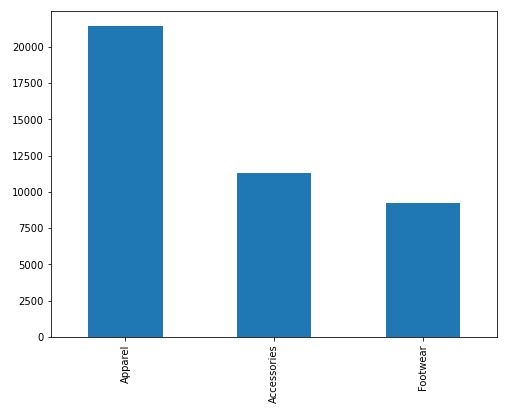
\includegraphics[scale = 1.5]{fileanh/5.jpg}
        \caption{Số lượng mỗi lớp sau khi xử lý}
    \end{figure}
\end{center}

\begin{block}{Nhận xét}
Bài toán này sẽ gồm có:
\begin{itemize}
    \item 41906 hình ảnh đã được gán nhãn 
    \item 3 lớp chính với số lượng như sau:
    \begin{itemize}
        \item Apparel \ \ \ \ \ \ \ 21395
        \item Accessories \ \ 11289
        \item Footwear \ \ \ \ \ \ \ 9222
    \end{itemize}
\end{itemize}
\end{block}
\newpage